\begin{frame}{Using upper ontologies}{Fixing a cim:Outage (according to nen-2660) }

    \AddToShipoutPictureFG*{
    \AtPageUpperLeft{\put(-5,-15){\makebox[\paperwidth][r]{Requirement 3}}}
    }%

    \begin{columns}[T] % align columns
        \begin{column}{.48\textwidth}
        \begin{figure}
            \centering
            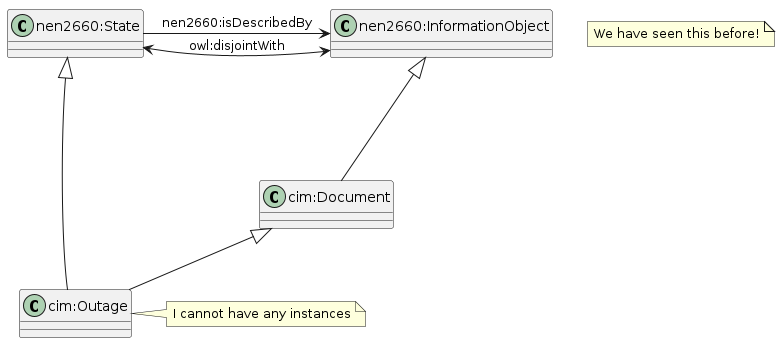
\includegraphics[width=1\textwidth]{slides/alignment/fixing-cim-outage/figs/AutageNaiveAttempt.png}
            \caption{Outage as State \textit{and} InformationObject}
        \end{figure}
        \end{column}%

        \begin{column}{.48\textwidth}
            \begin{figure}
                \centering
                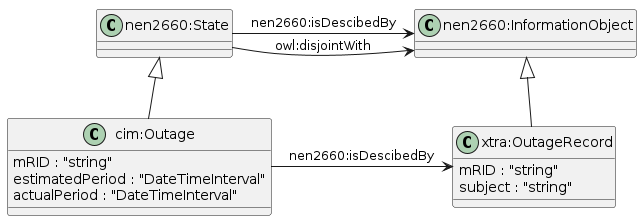
\includegraphics[width= 0.9 \textwidth]{slides/alignment/fixing-cim-outage/figs/FixingOutage.png}
                \caption{Separating the state from the record that describes it}
                \label{fig:FixingOutage}
            \end{figure}
        \end{column}
    \end{columns}
\end{frame}
